% !TeX spellcheck = de_DE
\section{Methodik}
\label{sec:Methodik}

	\subsection{Datensatz}
	\label{ssec:Datensatz}

	    Der für die Modellwahl verwendete Datensatz beinhaltet die logarithmierten relativen Reflexionswerte $\delta(\lambda)$ bei Wellenlängen zwischen 1400 nm und 2672 nm in einem Abstand von 4 nm sowie die Stoffmengeanteile $y^\m{(N)}$, $y^\m{(SOC)}$ und entsprechenden pH-Werte von insgesamt 533 Proben.
	    Für diese Arbeit sind lediglich die gegeben Reflexionswerte und der Stoffmengenanteil des Stickstoffes von Interesse.

	    Informationen über die chemische Zusammensetzung der Probe in den Reflexionswerten im Nahinfrarotbereich sind stark überlagert.\cite{Agelet2010}
	    Aus diesem Grund ist eine sorgfältige Auswahl relevanter Wellenlängen von besonderer Bedeutung für die Erstellung eines zuverlässigen Modells.


	% subsection Datensatz

	\subsection{Statistisches Modell}
	\label{ssec:Statistisches Modell}

	    Sei $n\in\SN$ die Größe des Datensatzes und $d\in\SN$ mit $d< n$ die Anzahl der Wellenlängen im Datensatz.
	    Entsprechend Abschnitt \ref{ssec:Nahinfrarotspek} definieren wir dann die Einflussgröße $x_{ik}$ für die $i$te Probe und $k$te Wellenlänge als
	    \[
			x_{ik} \define -\log \delta_i(\lambda_k)
		\]
		für jedes $i,k\in\SN,i\leq n,k\leq d$.

	    Der Stoffmengenanteil des Stickstoffs  $y^\m{(N)}$ stellt eine Ausprägung der Zielgröße unseres späteren Modells dar.
	    Wir definieren hierfür den Vektor der Stoffmengenanteile $y_i$ der $i$ten Probe als den $n$-dimensionalen Vektor
		\[
			 y \define \curvb{y^\m{(N)}_i}
		\]

        Nachdem wir sowohl die Einflussgrößen als auch die Zielgröße für das lineare Modell definiert haben, lassen sich diese nun in Zusammenhang bringen.
        Es ist valide anzunehmen, dass sich die Zielgröße durch einen Linearkombination der Einflussgrößen beschreiben lässt.
        Hierfür definieren wir zunächst $Y$ als einen zufälligen Vektor von $y$ mit
        \[
			 \expect Y \define \beta_0 + \sum_{j=1}^k{x_{ik}\beta_j}
		\]

		Zudem ist es notwendig eine Variable $\varepsilon$ einzuführen welchen den Zufall der Messungen beschreibt.
	    In Matrixschreibweise lässt sich dies durch die Designmatrix $\mathbb{X} \in \SR^{n \times (d+1)}$, dem Parametervektor $\beta \in \SR^{d+1}$ und dem stochastisch  verteilten Parameter $\varepsilon$ wie folgt darstellen.
		\[
			Y = \mathbb{X}\beta + \varepsilon
		\]
		Für den Zufallsparameter $\varepsilon$ wird weiterhin gefordert, dass
		\[
			\expect \varepsilon = 0, \qquad \cov \varepsilon = \sigma^2 \idmat
		\]
		wobei $\sigma^2 \in (0,\infty)$.
		Weiterhin soll angenommen werden, dass $\varepsilon$ normalverteilt ist mit
	    \[
			\varepsilon \sim \FN \curvb{0,\sigma^2\idmat}
		\]
	    sodass sich für das Gesamtmodell gilt
		\[
			Y \sim \FN \curvb{\mathbb{X}\beta,\sigma^2 \idmat}
		\]
      

	% subsection Statistisches Modell

	\subsection{Modellwahl im Falle der NIR-Spektroskopie}
	\label{ssec:modellwahl_nir}
	Seien $Y\in \rm I\!R^{n}$ die Zielgröße in einem statistischen Modellwahlverfahren und $\mathbb{X} \in \rm I\!R^{n \times d}$ eine Designmatrix.
	Zur Wahl einer geeigneten Menge von $k$ Einflussparametern auf die Zielgröße $y_i$  wird klassischerweise die Modellwahl über eine hierarchische Aufstellung von linearen Modellen erreicht. 
	Beginnend mit dem minimalen Modell $E(Y_i) = \beta_0$ werden nach und nach neue potenzielle Einflussparameter $x_{ik}$ hinzugefügt. 
	Zu jedem dieser neuen $x_{ik}$ wird dann eine Teststatistik aufgestellt, die darauf hinweist, ob der gewählte Parameter wichtig ist ist oder nicht. 
	Dabei ist die Nullhypothese, dass $x_{ik}$ keinen Einfluss auf die Zielgröße hat: $ H_0 = \beta_k = 0$ und wird abgelehnt, falls $H_1 = \beta_k \neq 0$ zutrifft.
	Dies wird über die T-Teststatistik erreicht,  wobei für den Fall, dass $H_0$ richtig ist, gilt:
	\begin{align*}
		\frac{\hat{\beta_k}}{\sqrt{\sigma^2(\mathbb{X}^T\mathbb{X})^{-1}_{kk}}} \sim t_{n-(k+1)}.
	\end{align*}
	Dieses Verfahren ist vor allem dann besonders gut geeignet, wenn man bereits theoretisch fundierte Annahmen über die Einflussgrößen machen kann.
	Mit diesem Modellwahlverfahren ergeben sich hier allerdings einige Schwierigkeiten:
	Durch die große Anzahl potenzieller Einflussgrößen im Form von Reflexionswerten kann a priori nur schwer eine inhaltliche Deutung vorgenommen werden.
	Daher ist Identifizierung weniger wichtiger Einflussgrößen und somit eine effektive hierarchische Modellwahl nicht möglich. 
	Demnach muss in dieser Arbeit die Anzahl der möglichen Einflussgrößen stark erhöht werden und hier bekommen wir ein Problem mit der T-Teststatistik. 
	Es ließen sich sehr viele unterschiedliche Kombinationen von Einflussgrößen aufstellen und in eine hierarchische Form bringen. 
	Doch da wir bei der T-Teststatistik ein \textit{zufälliges} Intervall konstruieren, gegen das unsere Hypothese getestet wird, wird die Wahrscheinlichkeit bei oft wiederholten Tests fälschlicherweise die Nullhypothese abzulehnen mit Anzahl der Versuchen immer größer. 
	Ein automatisiertes Modellwahlverfahren, das in dieser Arbeit von Vorteil ist, ist also mittels des T-Tests nicht zu erreichen \cite{Schumacher.2019}.
	Stattdessen bietet sich eine Modellwahl basierend auf dem erwarteten Prognosefehler ("sum of prediction squared error", SPSE) an:
	\begin{align*}
		SPSE \define \expect(\sum_{i=1}^{n} (Y_{i+n} - \hat{Y_i}^{(M)})^2)
	\end{align*}
	Hierbei sind die Werte in $Y_{i+n}$ neue Beobachtungen zum Erwartungsvektor $x_i$ und $\hat{Y_i}^\m{(M)}  = x_{i}^\m{(M)}\hat{\beta_i}^\m{(M)}$ die Prognosewerte aus dem zu testenden Modell $M$.
	Der Prognosefehler lässt sich in 3 Terme zerlegen: Einen irreduzierbaren Prognosefehler, der unabhängig von dem momentan betrachteten Modell ist, einen Biasterm, der die Abweichung des aktuellen Modells $M$ vom Prognosemodell als Summe der quadrierten Prognose-Verzerrungen anzeigt und einen Varianzterm, der die Ungenauigkeiten widerspiegelt, die sich aus der Schätzung von $p = (|M|+1)$ unbekannten Parametern ergibt:
	\begin{align*}
		SPSE^\m{(M)} = n\sigma^2 + p\sigma^2 + (bias^\m{(M)})^2
	\end{align*}
	Der SPSE lässt sich über unterschiedliche Wege schätzen: \\(1) mithilfe neuer Beobachtungen, \\(2) (wiederholter) Zerlegung der Ursprungsdaten in Test- und Trainingsdaten (Kreuzvalidierung)  oder \\(3) mittels Schätzung basierend auf der Residuenquadratsumme ("residual squared sum", RSS), hier im Vergleich zu o.g. SPSE:

	\begin{align*}
	RSS^{(M)} \define \sum_{i=1}^{n} (Y_{i} - \hat{Y_i}^{(M)})^2
	\end{align*}
	\begin{align*}
	SPSE^{(M)} \define \sum_{i=1}^{n} \expect (Y_{i+n} - \hat{Y_i}^{(M)})^2
	\end{align*}
  Es kann gezeigt werden, dass RSS den Wert von SPSE systematisch unterschätzt, dies jedoch durch die Verwendung der geschätzten Varianz des maximalen Modells behoben werden kann.\cite{Schumacher.2019}:
	\begin{equation}\label{eq:spse_true}
	SPSE^\m{(M)} := RSS^\m{(M)} + 2 \tilde{\sigma}_{full} ^2 (k+1)
	\end{equation}
	Die Minimierung des SPSE entspricht der Minimierung des Mallow's Cp- Kriteriums, das für die folgenden Analysen getestet werden soll. Dabei gilt:
	\begin{align*}
	C^\m{(M)}_p = \frac{1}{\sigma_\m{full}^2} \sum_{i=1}^\m{n} (y_i - \hat{y_i}^\m{(M)})^2 - n + 2(k+1)
	\end{align*}

	\subsection{Modellselektion}
	\label{ssec:modellselektion}
	Sei $\Lambda$ das Spektrum der erhobenen Wellenlängen im vorliegenden Datensatz.
	Das erste Ziel dieser Arbeit ist es, diejenigen Wellenlängen $\lambda\in\Lambda$ herauszufinden, deren Reflektionswerte $x_j$ durch den vom Stickstoffgehalt der beeinflusst werden.  
	Es wurden mehrere Selektionsverfahren verglichen, die auf zwei Annahmen basieren: \\
	(1) Die erste Ableitung $x_j'$ der Reflexionswerte zeigt an deren \textit{Veränderungen} an über das gesamte Spektrum an. 
	Da bei der großen Anzahl an potenziellen Einflussgrößen eine Vorauswahl schwierig ist, wurden also diejenigen mit auffälligem mathematischen Verhalten ausgewählt: (a) diejenigen Reflexionen, deren 1. Ableitung über einem Schwellwert $\tau_1$ lag oder (b) diejenigen, deren Werte unterhalb eines Schwellenwertes lagen.\\
	(2) Darüber hinaus wurden diejenigen Wellenlängen ausgewählt, die eine hohe Variablilität $var(x_j') > \tau_2$ aufweisen. 
	Zur Berechnung der Variablilität wurden wiederum unterschiedliche Verfahren angewandt. In Modell (a) wurde die Differenz zwischen dem minimalen und dem maximalen Ableitungswert normaiert auf den Mittelwert, während (b) und (c) ohne Normierung arbeiten. In (b) wird lediglich zusätzlich der Betrag verwendet: 	\\ \\
	(a) $var(x_j') = \frac{|max(x_j') - min(x_j')|}{mean(x_j')}$\\
	(b) $var(x_j') = |max(x_j') - min(x_j')|$\\
	(c) $var(x_j')= max(x_j') - min(x_j')$\\ \\
	Der Vergleich zwischen den Modellen ergab, dass der SPSE am kleinsten wird, wenn wir diejenigen Reflexionen verwenden, deren erste Ableitung und Variablilität über $\tau_1$, liegt. (2b), oder:
	\begin{align*}
		X_{select} = \{x_j' \in \Lambda |max(x_j') - min(x_j')| > \tau_1\}
	\end{align*}

%	\begin{figure*}
%		\label{Wellenlängen_erste_Ableitung}
%		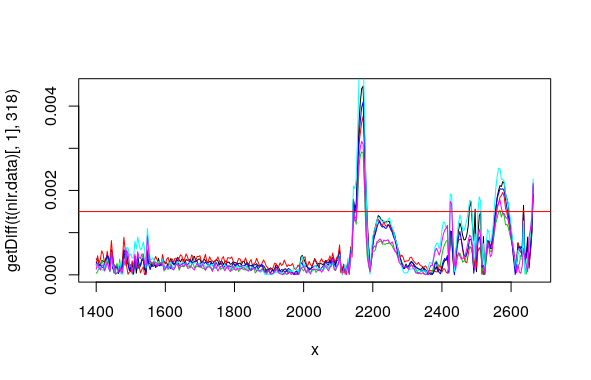
\includegraphics[width=\textwidth]{img/wave_1dev.png}
%		\caption{Ableitungen der Wellenlängen von fünf zufälligen Spektren}
%	\end{figure*}

	Die so ausgewählten Wellenlängen wurden als Maximalmodell in der Berechnung von Mallow's $C_p$ gegeben. Da immer noch sehr viele Variablen im Modell sind, wurde die performantere Rückwärtsselektion für die konkrete Berechnung verwendet.

	\subsection{Validierung des Modells}
	\label{ssec:model-validation}
	   Ein Parameter zur Messung der globalen Anpassungsgüte einer Regression ist $R^2$, definiert als \cite{Lang2007}
		\[
			{R^2}^{(M)} \define \frac {\sum_{i=1}^n \curvb{\hat{y}^{(M)}_i - \overline{y}}^2}{\sum_{i=1}^n \curvb{y_i - \overline{y}}^2}
		\]
		Dieser beschreibt den Anteil der durch die Regression erklärten Varianz in den Daten und nimmt Werte zwischen 0 und 1 an.
		Während ein $R^2$ von 1 für einen perfekten linearen Zusammenhang steht bedeutet ein Wert von 0, dass kein linearer Zusammenhang vorliegt.
		Für das gewählte Modell ergibt sich ein Wert von $R^2 =  0.82$.
		Zudem ist es sinnvoll neben dem Parameter $R^2$ ein Korrelationsdiagramm zwischen der durch das Modell geschätzten Ausprägung $\hat{y}_i$ und dem wahren Wert $y_i$ zu betrachten. Dies ist in Abbildung \ref{fig:correlation} dargestellt.

	% subsection model-validation

	%\subsection{Assessment by Simulation}
	%\label{ssec:simulation}


	\subsection{Theoretische Grundlagen der Simulation}
	\label{ssec:Theoretische Grundlagen der Simulation}

        Wie in Abschnitt \ref{ssec:modellwahl_nir} beschrieben gibt der SPSE den erwarteten Prognosefehler an.
        Es ist offensichtlich, dass dieser Wert möglichst gering sein sollte, um ein verlässliche Vorhersagen zu neuen Daten zu generieren.

        Im Allgemeine kann der SPSE mit Hilfe neuer Beobachtungen geschätzt werden.\cite{Schumacher Skript}
        Da diese nicht zur Verfügung stehen werden stattdessen neuen Pseudobeobachtungen der Zielgröße mit Hilfe des gewählten Modells generiert.
        Der aus der Pseudobeobachtungen geschätzte Prognosefehler kann der mit dem wahren wahren Prognosefehler des Modellsverglichen werden.
        Bei gegebenem Modells $M$ wird der wahre Prognosefehler durch
        \[
            SPSE^\m{(M)} \define  n \sigma^2 + \curvb{\abs{M}+1} \sigma^2
        \]
        berechnet.

        Der neue Vektor der Pseudobeobachtungen ist gegeben durch,
        \[
            \widetilde{Y} \define \widetilde{y}_i + \varepsilon
        \]
        wobei für den stochastisch verteilen Parameter $\varepsilon$ gilt
        \[
            \varepsilon \sim \FN \curvb{0,\sigma^2\idmat}
        \]
        und als Varianz die Varianz des Modells angenommen wird.
        \[
            \sigma^2 \define \curvb{\tilde{\sigma}^2}^{(M)}
        \]
        Aus den generierten Pseudodaten wird ein neues bestes Modell $\widetilde{M}$ auf basierend auf dem kleinsten Cp-Wert ausgewählt, für dass gilt.
        \[
            \widetilde{Y} \sim \FN \curvb{\mathbb{X}^\m{(\widetilde{M})}\widetilde{\beta}, \sigma^2 I}
        \]
        Hierfür wird die Varianz als unbekannt angenommen.
        Neben dem Vergleich des wahren und geschätzten Prognosefehlers bei gleicher Stichprobengröße soll zudem überprüft werden welcher Einfluss die Änderung der Stichprobengröße auf den Wert des geschätzten SPSE hat.
        Hierzu werden die verschiedenen Stichprobengrößen von $n = (150, 200, 250, 300, 350, 400, 450, 500, 533)$ gewählt und zufällig aus dem Datensatz ausgewählt.
        Um die Verzerrung der Ergebnisse durch zufällige Ausreißer zu vermeiden werden die Simulationen mehrfach durchgeführt.


	% subsection Theoretische Grundlagen der Simulation
% section methodology
